%

\begin{figure*}[!ht]
    \centering
  \begin{minipage}{0.31\textwidth}
    \centering
    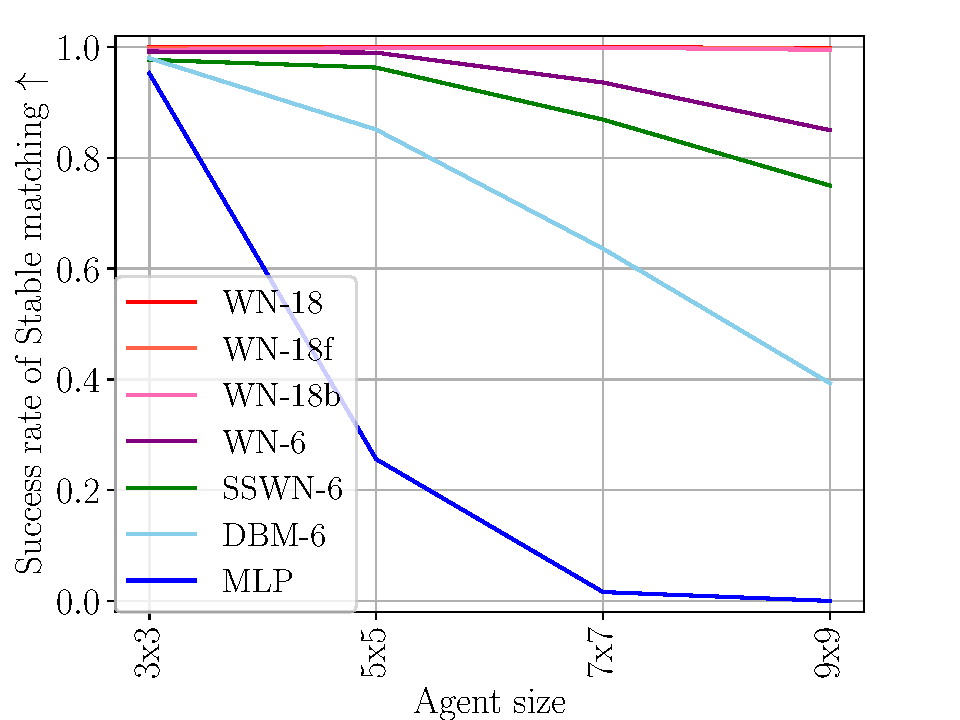
\includegraphics[width=1.0\linewidth]{figures/Fig4_sm.pdf}
    \caption{Change in the success rates of stable matching ($\uparrow$) according to $N$.~\newline}
    \label{fig:Ex1_a}
  \end{minipage}%
  \begin{minipage}{0.035\textwidth}~
  \end{minipage}%
  \begin{minipage}{0.31\textwidth}
    \centering
    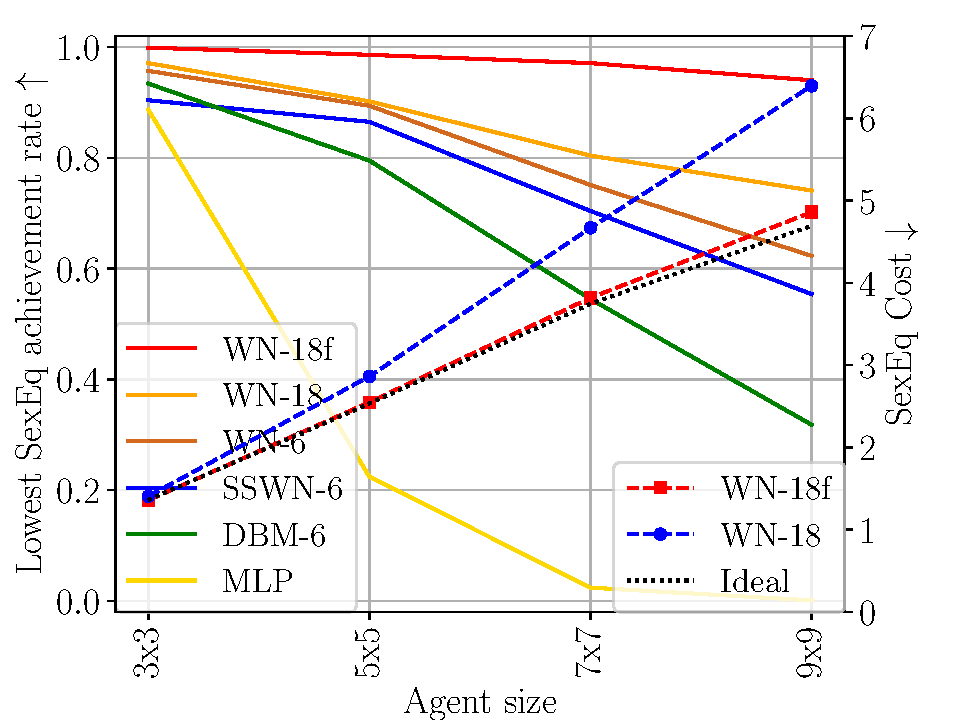
\includegraphics[width=1.0\linewidth]{figures/Fig5_SEqCost.pdf}
    \caption{The rates of achieving the ideal fair-stable matching with minimum $\SEq$ (solid, $\uparrow$), and the average $\SEq$ (dashed, $\downarrow$).}
    \label{fig:Ex1_b}
  \end{minipage}%
  \begin{minipage}{0.035\textwidth}~
  \end{minipage}%
  \begin{minipage}{0.31\textwidth}
    \centering
    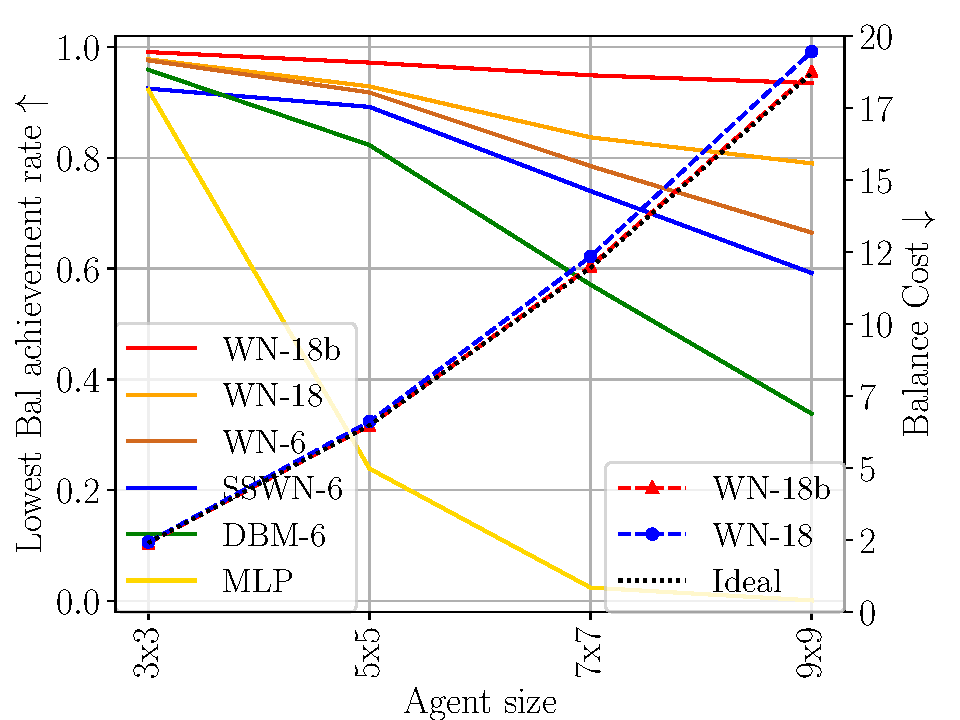
\includegraphics[width=1.0\linewidth]{figures/Fig6_BalCost.pdf}
    \caption{The rates of achieving the ideal fair-stable matching with minimum $Bal$ (solid, $\uparrow$), and the average $Bal$ (dashed, $\downarrow$).}
    \label{fig:Ex1_c}
  \end{minipage}%
\end{figure*}


\section{Experiments}\label{s:exp}
We evaluated WeaveNet through two experiments and one demonstration.
First, with test samples of $N<10$, we compared its performance with learning-based baselines and optimal solutions obtained by a brute-force search.
Second, we compared WeaveNet with algorithmic baselines at $N=20,~30$.
Third, we demonstrate its performance at $N=100$. Note that we always assume $M=N$ hereafter. 

\subsubsection{Sample Generation Protocol}
In the experiments, we used the same method as \cite{tziavelis2019equitable} to generate synthetic datasets that draw preference lists from the following distributions. 
\setlength{\leftmargini}{3pt}{
\begin{description}
\item[Uniform (U)] Each agent's preference towards any matching candidate is totally random, defined by a uniform distribution $\mathcal{U}(0,1)$ (larger value means prior in the preference list).
\item[Discrete (D)] Each agent has a preference of $\mathcal{U}(0.5,1)$ towards a certain group of $\lfloor 0.4N\rfloor$ popular candidates, while $\mathcal{U}(0,0.5)$ towards the rest.
\item[Gauss (G)] Each agent's preference towards $i$-th candidate is defined by a Gaussian distribution $\mathcal{N}(i/N,0.4)$. 
\item[LibimSeTi (Lib)] Simulate real rating activity on the online dating service LibimSeTi \cite{brozovsky07recommender} based on the 2D distribution of frequency of each rating pair ($p^A_{ij},~p^B_{ji}$).
\end{description} 
}

Choosing the above preference distributions for group $A$ and $B$ respectively, we obtained five different dataset settings, namely UU, DD, GG, UD, and Lib.
We randomly generated 1,000 test samples and 1,000 validation samples for each of the five distribution settings.

\subsubsection{Training Protocol}
We trained any learning-based models 200k total iterations at $N\leq 30$ and 300k at $N=100$, with a batch size of $8$\footnote{The number of training samples is $3.7\times 10^{-9}$\% of total cases even when $N=5$ and the overlap with test samples is negligible.}. 
We randomly generated training samples at each iteration based on the distribution of each dataset and used the Adam optimizer \cite{adam}.
We set learning rate 0.0001 and loss weights $\lambda_s=0.7$, $\lambda_m=1.0$, $\lambda_f=\lambda_b=0.01$ based on a preliminary experiment (see \ref{app:hyperparameters}). 

\subsection{Comparison with Learning-based Methods}\label{ss:exp1}

%\subsubsection{Baselines and Ablations}
In this experiment, we show results obtained by following baselines and WeaveNet variants.
{\bf MLP} is the model proposed in \cite{harvard2019}. 
{\bf DBM-6} is Deep Bipartite Matching \cite{gibbons2019deep} with $L=6$ layers.
{\bf SSWN-6} is the single-stream WeaveNet with $L=6$ layers.
This variant is to test how WeaveNet works when adopting the single-stream design of DBM.
{\bf WN-6} and {\bf WN-18} is the standard WeaveNet with $L=6$ and $L=18$ layers, respectively.
All the above models were trained to optimize Eq.~\eqref{eq:lsm}. 
{\bf WN-18f} and {\bf WN-18b} have the same architecture with WN-18, but were trained to optimize Eq.~\eqref{eq:lfsm} and Eq.~\eqref{eq:lbsm}, respectively. 
Note that MLP was trained for each $N$ because the network cannot flexibly accept different-size problem instances. The other methods were trained with samples of $N=10$ and tested on samples of $N=3,~5,~7,~9$.
Models with $L=6$ have a similar number of parameters with the MLP model (for sample size $N=5$), so they can have a fair comparison of parameter efficiency. WN models with $L=18$ are aimed to show a larger potential.
See \ref{ss:exp1_supp} for more precise definition of each architecture.

%\subsubsection{Results}
Fig.~\ref{fig:Ex1_a} shows the success rates of finding a stable matching. MLP can hardly find stable matchings when $N\geq 5$. DBM performs better than MLP but still obviously worse than any of WeaveNet variants. Standard WeaveNet's two-stream architecture shows advantages over its single-stream variant.

Fig.~\ref{fig:Ex1_b} and \ref{fig:Ex1_c} show the success rates of finding the possibly fairest (i.e., lowest $\SEq$ or $Bal$) stable matching (solid lines) and the average costs of $\SEq$ and $Bal$ (dashed lines), respectively. Each method has the same trend of performance as in Fig.~\ref{fig:Ex1_a}.
Specifically, the gap between WN-18 and WN-18f/b proved the flexibility of the model for customizing the objective function.

%%%%%%%%%%%%%%%%%%%%%%%%%%%%%%%%%%%%%%%%%%%%%%%%%%%%%%%%%%%%%%%%%
\begin{table*}[ht!]
\setul{1pt}{.4pt}
 \begin{center}
 \setlength\tabcolsep{6pt} % セルの左右の余白
 \scalebox{1.0}{
 \small
  \begin{tabular}{lrrrrr|rrrrr} \toprule
      %\multicolumn{13}{|c|}{SEq Cost } \\ \hline
      Agents ($N\times M$) & \multicolumn{5}{c}{$20 \times 20$ } & \multicolumn{5}{|c}{$30 \times 30$ } \\ %\midrule
      Datasets (Distribution Type) & \multicolumn{1}{c}{UU}    & \multicolumn{1}{c}{DD}    & \multicolumn{1}{c}{GG}    & \multicolumn{1}{c}{UD}     & \multicolumn{1}{c}{Lib}    & \multicolumn{1}{|c}{UU}    & \multicolumn{1}{c}{DD}    & \multicolumn{1}{c}{GG}    & \multicolumn{1}{c}{UD}     & \multicolumn{1}{c}{Lib} \\ \midrule
      GS                 & 41.89 & 18.81 & 19.52 & \ul{\bf 70.97}  & 19.66 & 94.03 & 43.46 & 36.56 & \ul{163.77} & 39.78  \\
      PolyMin            & 19.93 & 11.83 & 20.57 & 87.08  & 18.47 & 35.52  & 21.21 & 37.37 & 209.62 & 31.85  \\
      DACC               & 24.34 & 20.13 & 23.07 & 101.75 & 20.40 & 40.87  & 34.35 & 40.59 & 240.48 & 33.88  \\ 
      Power Balance      & \ul{16.28} & \ul{8.93}  & \ul{17.07} & 71.09  & \ul{15.40} & \ul{18.45}  & \ul{11.05} & \ul{27.22} & 163.90 & \ul{21.57}  \\ 
      \midrule
      WN-60f (Ours) & {\bf 11.44} & {\bf 6.32}  & {\bf 15.34} & 71.18 & {\bf 14.44} & {\bf 16.07} & {\bf 9.64}  & {\bf 26.46} & {\bf 162.61} & {\bf 21.29} \\
      Stable Match (\%)   & 99.10 & 99.40 & 99.40 & 99.50 & 99.80 & 98.10 & 99.00 & 98.00 & 93.90  & 98.60 \\ 
      \midrule
      Win (\%)            & {\bf 25.90} & {\bf 29.70} & {\bf 12.20} & 0.00  & {\bf 9.50}  & {\bf 14.60} & {\bf 25.30} & 9.30  & 0.10   & 8.00  \\
      Tie (\%)            & 67.30 & 60.60 & 83.20 & 96.70 & 86.20 & 72.30 & 54.70 & 78.10 & 89.20  & 80.80 \\
      Loss+Unstable (\%)   & 6.80  & 9.70  & 4.60  & {\bf 3.30}  & 4.30  & 13.10 & 20.00 & {\bf 12.60} & {\bf 10.70}  & {\bf 11.20} \\
      %\hline \hline
      \bottomrule
    \end{tabular}
    }
    \caption{Average $\SEq$ ($\downarrow$), success rate of stable matching, and winning/losing rate against the best algorithmic method (underlined). }
    \vspace{1.0em}
    \label{table:SEqCost}
    
    \scalebox{1.00}{
    \small
    \begin{tabular}{lrrrrr|rrrrr} \toprule
      %\multicolumn{13}{|c|}{Balance Cost } \\ \hline
      Agents ($N\times M$) & \multicolumn{5}{c}{$20 \times 20$ } & \multicolumn{5}{|c}{$30 \times 30$ } \\ %\midrule
      Datasets (Distribution Type) & \multicolumn{1}{c}{UU}    & \multicolumn{1}{c}{DD}    & \multicolumn{1}{c}{GG}    & \multicolumn{1}{c}{UD}     & \multicolumn{1}{c}{Lib}    & \multicolumn{1}{|c}{UU}    & \multicolumn{1}{c}{DD}    & \multicolumn{1}{c}{GG}    & \multicolumn{1}{c}{UD}     & \multicolumn{1}{c}{Lib} \\ \midrule
      GS                 & 89.14 & 146.16 & 108.36  & \ul{\bf 140.53} & 68.62 & 184.05 & 322.05 & 225.49 & \ul{\bf 312.12} & 137.59 	 \\ % 312.119
      PolyMin            & 74.19  & 140.99 & 108.04 & 145.28 & 66.94 & 144.48 & 306.28 & 224.13 & 324.54 & 130.79 	\\
      DACC               & 78.49  & 146.71 & 110.06 & 151.34 & 68.75 & 150.71 & 316.18 & 227.52 & 337.43 & 133.59 	\\ 
      Power Balance      & \ul{73.28}  & \ul{140.12} & \ul{106.92} & 140.55 & \ul{65.89} & \ul{138.04} & \ul{302.30} & \ul{\bf 220.26} & {\bf 312.12} & \ul{\bf 126.96} 	\\ %312.123
      \midrule
      WN-60b (Ours) & {\bf 71.29} & {\bf 138.57} & {\bf 106.50} & 140.72 & {\bf 65.63}  & {\bf 137.70}  & {\bf 301.08}  & 221.12  & 313.11  & 127.12 \\
      Stable Match (\%)   & 98.00 & 99.10  & 98.60  & 99.80  & 99.10  & 97.00   & 98.60   & 93.70   & 98.80   & 98.00 \\ \midrule
      Win (\%)            & {\bf 20.60} & {\bf 29.80}  & {\bf 9.40}   & 0.00   & 6.60   & 10.40   & {\bf 25.70}   & 6.20    & 0.10    & 5.60 \\
      Tie (\%)            & 69.50 & 63.70  & 81.90  & 95.00  & 86.60  & 71.60   & 63.20   & 69.50   & 83.90   & 81.50 \\
      Loss+Unstable (\%)   & 9.90  & 6.50   & 8.70   & {\bf 5.00}   & {\bf 6.80}   & {\bf 18.00}   & 11.10   & {\bf 24.30}   & {\bf 16.00}   & {\bf 12.90} \\
      \bottomrule
    \end{tabular}
    }
  \caption{Average $Bal$ ($\downarrow$), success rate of stable matching, and winning/losing rate against the best algorithmic method (underlined).}
  \label{table:BalCost}
     \end{center}
\end{table*}

\subsection{Comparison with Algorithmic Methods}\label{ss:exp2}
%Next, we compared WeaveNet with algorithm-based solvers.
%\subsubsection{Baselines and Learning Setting of WeaveNet}
%As the algorithmic approaches, we prepared four baselines.
{\bf GS} is the better result of applying the GS algorithm \cite{gale1962college} to prioritize each side once. {\bf PolyMin} is an algorithm that minimizes the regret and egalitarian costs (Table \ref{tab:costs}) instead of $\SEq$ and $Bal$ costs, which we can calculate in polynomial time.
{\bf DACC} \cite{dworczak2016deferred} is an approximate algorithm that runs in $O(n^4)$. {\bf PowerBalance} is the state-of-the-art method that runs in $O(n^2)$. 

{\bf WN-60f/b} is WeaveNet with $L=60$ layers. It was trained with samples of $N=30$ and tested on $N=20,~30$. 
Note that we used the asymmetric variant for UD and Lib. See \ref{ss:exp2_supp} for a detailed ablation study for the symmetric and asymmetric variants and so on.

%\subsubsection{Results}
We show the results in Tables \ref{table:SEqCost} and \ref{table:BalCost}.
In the $\SEq$ experiment, the proposed WN-60f achieved the best scores almost in all the cases, and narrowly lost in UD for $N=20$.
In the $Bal$ experiment, WN-60b also achieved the best scores in UU, DD, GG, and Lib for $N=20$ and UU, DD for $N=30$, and narrowly lost in the other four cases.
%WN-60f achieved the best $\SEq$ and $Bal$ in most settings in $\SEq$ scores. WN-60b similarily performed in $Bal$ scores, but only for $N=20$ and UU and DD for $N=30$.
Note that these scores of WN-60f/b involve unstable matchings.

To evaluate the results while strictly forbidding unstable matchings, we compared $\SEq$ and $Bal$ obtained by WN-60f/b with the best algorithmic method (underlined in the table) sample by sample, and counted win, tie, and loss percentages of WN, where unstable matchings were treated as losses.
Even with this setting, WN-60f beat the best algorithmic method in six among all the ten cases, and WN-60b won four among ten. To our best knowledge, other learning-based methods have never achieved such comparable results.
%Even with this setting, WN-60f/b won the best algorithmic method in UU, DD, GG for $N=20$ and DD for $N=30$, which have never been achieved by any other learning-based methods.

It is noteworthy that the asymmetric variant achieved a similar performance to the best algorithmic methods even in UD, the most biased setting, and Lib, the simulation of real preference distribution while keeping its parameter efficiency. % despite the weight sharing strategy. 

\begin{table}
\centering
{    \small
    \setlength\tabcolsep{4pt} % セルの左右の余白
    \begin{tabular}{lrr}
    \toprule
        \multicolumn{1}{c}{$100\times100$, UU} & \multicolumn{1}{c}{$\SEq$} & \multicolumn{1}{c}{$Bal$}  \\
        \midrule
        GS  & 1259.39 & 1709.53 \\  %116,736
        PolyMin  & 153.35 & 952.85 \\  %116,736
        DACC  & 194.65 & 988.02 \\  %116,736
        Power Balance & {\bf 49.41} & {\bf 909.73} \\  %116,736
        \midrule
        WN-80f/b+Hungarian & 68.36 & 919.75     \\  %68.356 919.747 %119,396
        Stable Match (\%) & 89.4 & 80.8 \\
        %\midrule
        %Win (\%)& {\bf 56.80} & 9.10 \\
        %Tie (\%)& 21.10 & 43.30 \\
        %Loss+Unstable (\%)& 22.10 & {\bf 47.60} \\
        % ちょっと，今レイアウトしているのでいじらないで欲しいです．
        \bottomrule
    \end{tabular}
}
    \caption{Average $\SEq$ ($\downarrow$) and $Bal$ ($\downarrow$) at $N=100$.}% WN-80f/b are used with the Hungarian algorithm.}
    \label{tab:N100_score}
\end{table}

%\begin{figure}[th]
%    \centering
%    \includegraphics[width=0.75\linewidth]{figures/Fig4_matchrate.pdf}
%    \caption{$N=100$の結果をまとめた図または表がここに入る予定.}
%    \label{fig:exp3}
%\end{figure}

\subsection{Demonstration with \texorpdfstring{$N=100$}{N=100}}
We further demonstrate the capability of WeaveNet under relatively large size of problem instances, $N=100$. In this case, we found that the binarization process ${\rm argmax}(\hat{m})$ of WeaveNet does not always successfully yield a one-to-one matching. Specifically, WN-80f and WN-80b found stable matchings for 84.4\% and 73.2\% samples while failed to yield one-to-one matchings for 13.4\% and 19.8\%, respectively (see the Table \ref{tab:N100_bp} in \ref{ss:exp2_supp} for details). To compensate for this problem, we applied the Hungarian algorithm to $\hat{m}$ to force an output of one-to-one matching. The results in Table \ref{tab:N100_score} demonstrate that WeaveNet still achieved a close performance to the state-of-the-art algorithmic method, under a problem size that other learning-based-method studies have never set foot into. We consider this result promising, and expect to further improve the scalability and the binarization reliability of WeaveNet.

%We further demonstrated WN-80f/b with samples from UU $N=100$.
%Table \ref{tab:N100_bp} shows how often the blocking pairs appear (i.e., unstable matching) in our test results.
%\jm{I kind of think that Table 4 is not very important to show here, use text description is fine. Then we can give more space to Table 5.}\ah{But we have no further data for Table 5...}\jm{Anyway the space is too tight for both Table 4 and Table 5. For Table 4, the ``WN-80f+Hung.'' will be more clear if we have space to write ``WN-80f $|$ WN-80f w. Hung.'', For Table 5, most algorithm names are highly abbreviated, and the row of GS does not have a proper interval so two values look like one.}
%In $N=100$ case, the ${\rm argmax}$binarization of $\hat{m}$ sometimes fails to output a one-to-one matching.
%\jm{could you add a reason here ``due to ...''?}\ah{I can expect the reason but cannot prove it based on data... maybe, it is due to the lack of model's discriminative capability to differentiate only one best partner-agent in each other in the 100:100 coupling candidates}
%Because we cannot calculate $\SEq$ and $Bal$ for such fail cases, we applied the Hungarian algorithm\cite{kuhn1955hungarian} to $\hat{m}$ to investigate how well we could optimize the fairness costs. The results in Table \ref{tab:N100_score} demonstrated that WeaveNet still works in this middle-size problem, although it does not always output one-to-one matchings.
%\jm{"although it may need an additional step of Hungarian algorithm to guarantee one-to-one matchings."}\ah{I think we do not need to guarantee one-to-one matchings, or we cannot guaranttee one-to-one matching even when $N<=30$.}\jm{I mean the current sentence ``...although it does not always output one-to-one matchings.'' looks uninformative, so I write a sentence to replace.}

